\chapter{Results of experiments with \nqp}
\label{app:nqp}
\textit{This Appendix, presents graphically a summary of individuals runs using \nqp. Figures show a \textit{box-plot} representation for different strategies and a bar representation for the percentage of winner solvers types.}

\vspace{2ex}\vfill
\minitoc
\newpage

\section{Comparison between sequential and parallel runs}

In Figures~\ref{boxplot:250}, \ref{boxplot:500}, \ref{boxplot:1000}, \ref{boxplot:3000} and~\ref{boxplot:6000}, labels of the x-axis correspond to the following strategies:

\poslcaptiondesciption{
\begin{tabular}[t]{rl}
\textbf{Seq}: & Sequential strategy (1 core)\\
\textbf{NC}: & Parallel non communicative strategy\\
\textbf{Cyc1-1}: & Cyclic communicating strategy with communication \oneTone \\
\textbf{Cyc1-n}: & Cyclic communicating strategy with communication \oneTn \\
\textbf{S1-1}: & Simple communicating strategy with communication \oneTone \\
\textbf{S1-n}: & One set of solvers performing a simple communicating strategy with communication \oneTone \\
\textbf{S1-n/2}: & Two sets of solvers performing a simple communicating strategy with communication \oneTone \\
\textbf{S1-n/4}: & Four sets of solvers performing a simple communicating strategy with communication \oneTone \\
\end{tabular}
}

\begin{wrapfigure}{R}{0.4\textwidth}
\centering
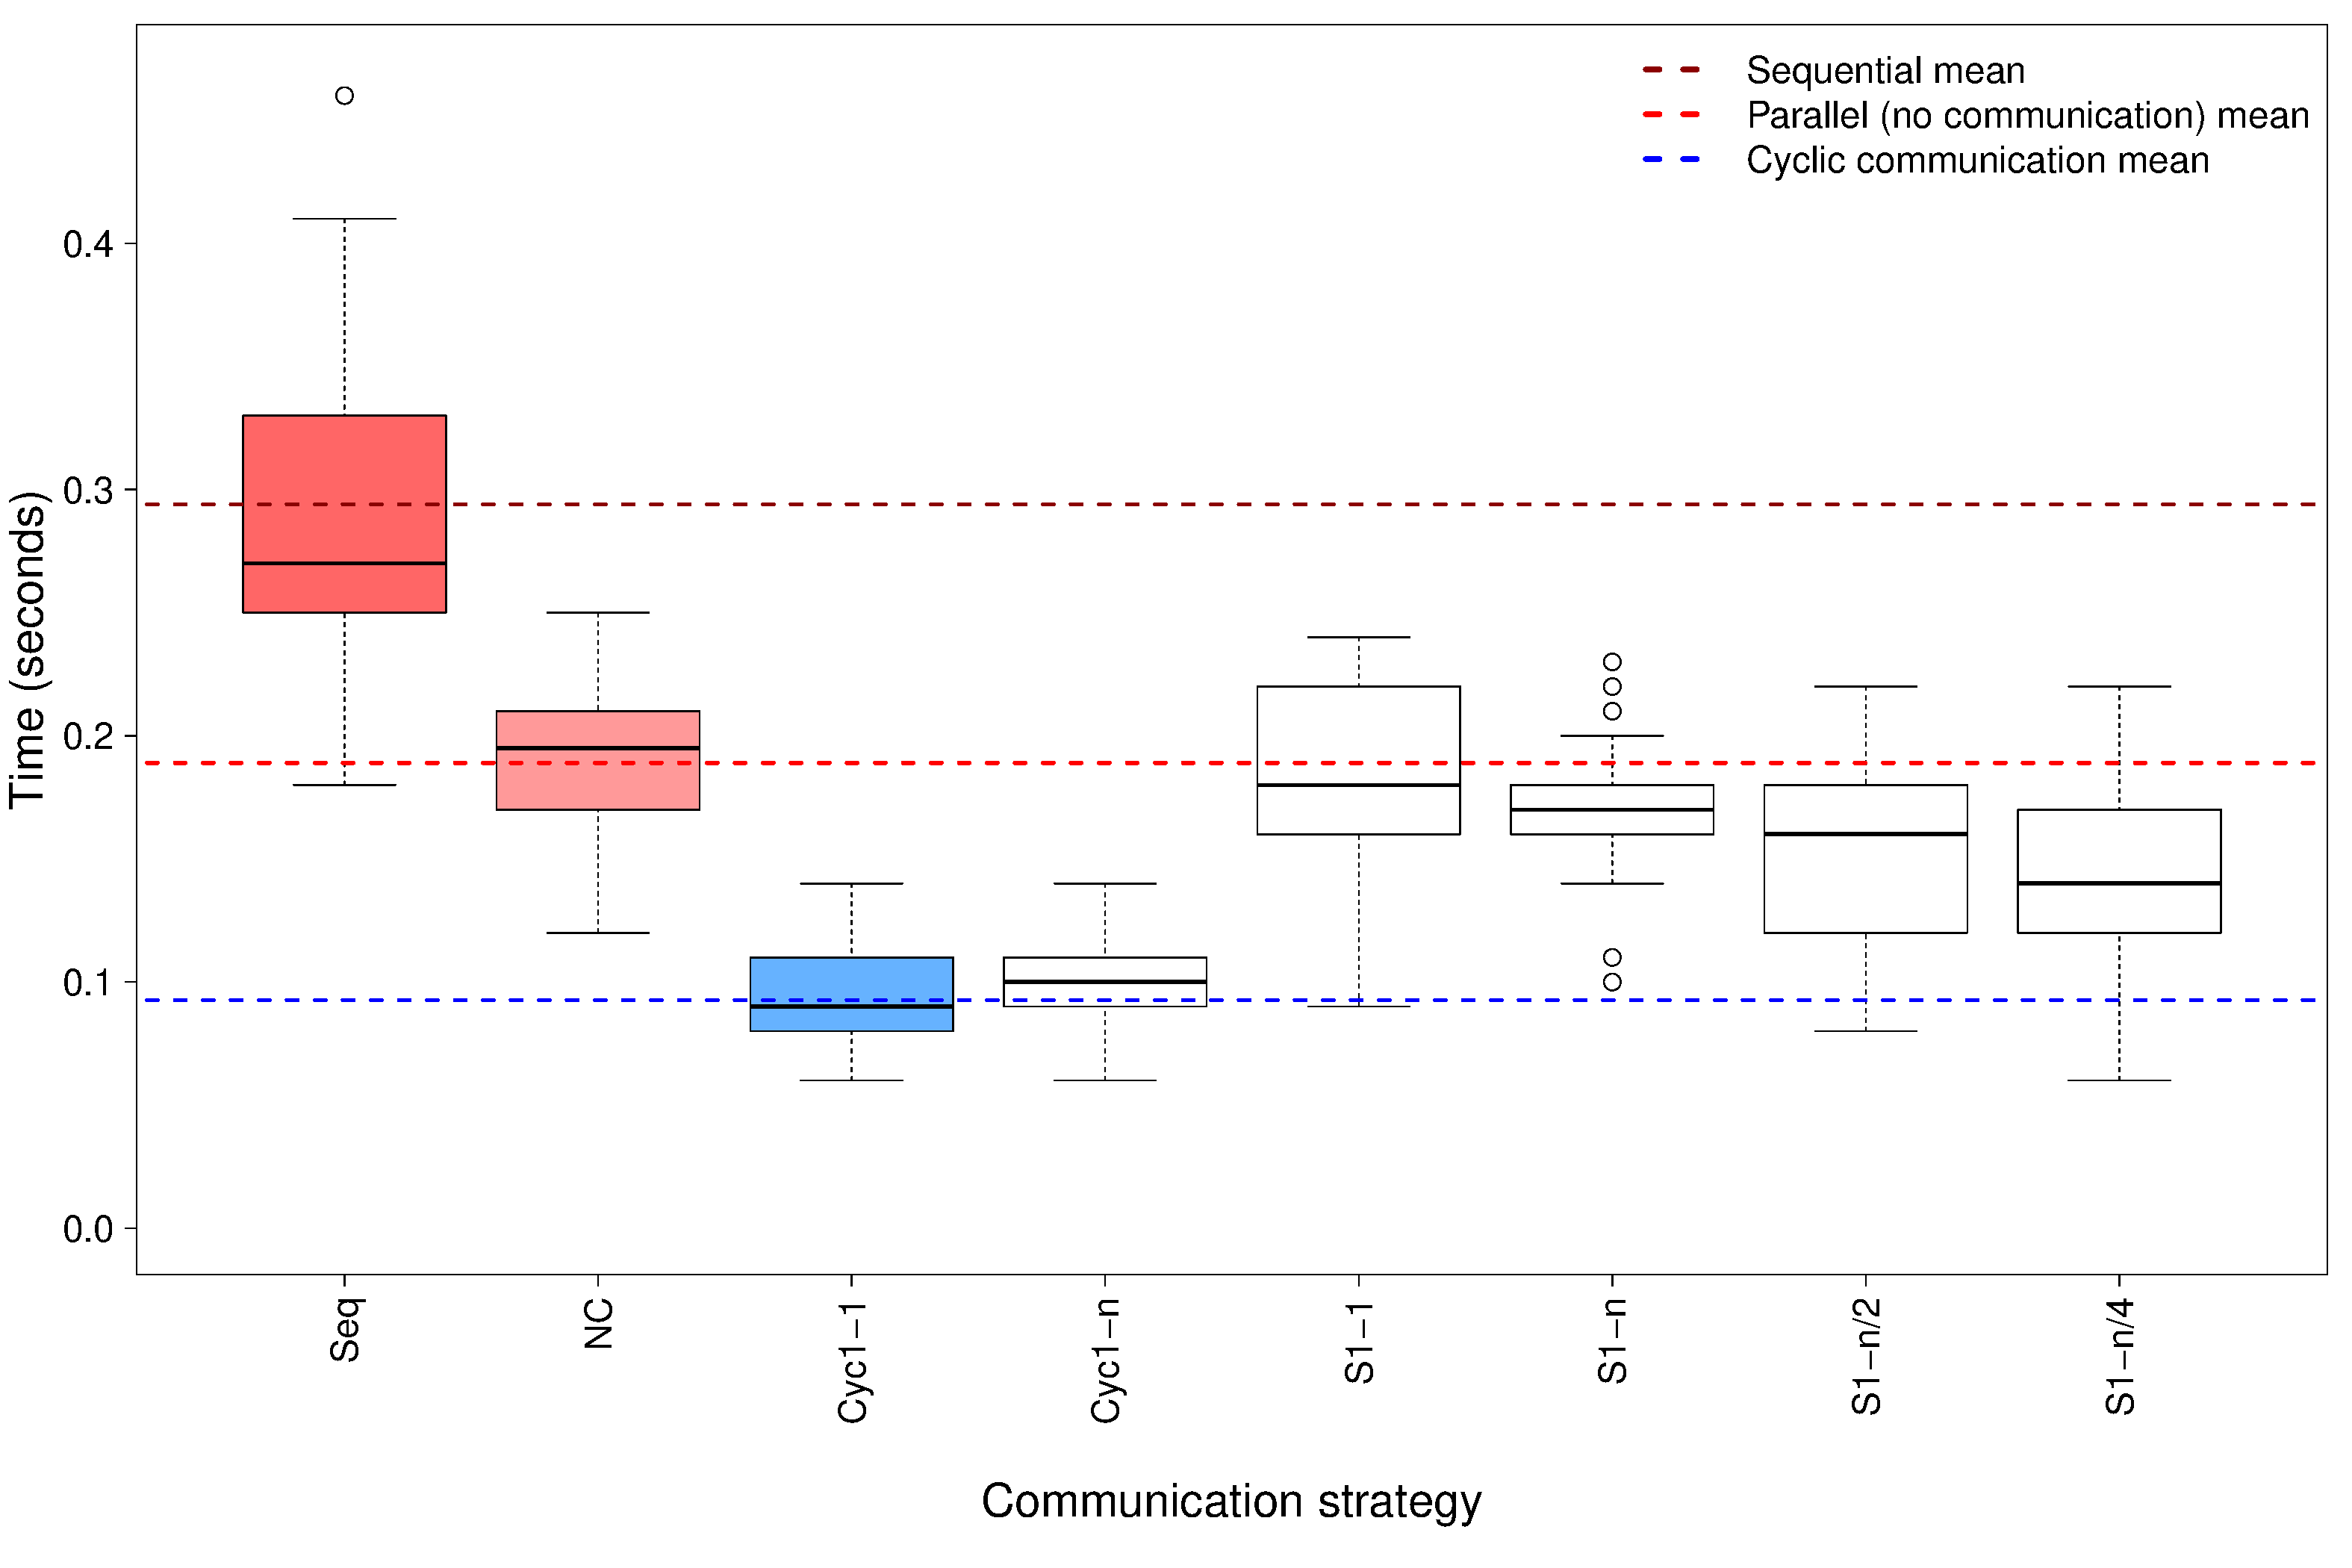
\includegraphics[width=0.35\textwidth]{nq250_BP.pdf}
\caption{Different communication strategies to solve 250-Queens using \posl}\label{boxplot:250}
\end{wrapfigure}

Figures~\ref{boxplot:250}, \ref{boxplot:500}, \ref{boxplot:1000}, \ref{boxplot:3000} and~\ref{boxplot:6000} show summaries of runs from the experimentation with \nqp{} using box-plot representation. They show sequential runs (\texttt{Seq}), parallel without communication runs (\texttt{NC}) and runs from the different \commstrs{} proposed.

As explained before in Chapter~\ref{chap:expe}, in these graphs can be observed from another point of view how the best found \commstr{} contribute less in terms of runtime when the problem order ($N$: the number of queens) increases. They also show that simple \commstrs{} do not work for this problem: their results are better (lower runtimes) but not competitive.

For the smaller instance, the cyclic \commstr{} work very well. The graph in Figure~\ref{boxplot:250} shows how for both strategies (\texttt{Cyc1-1} and \texttt{Cyc1-n}) all runtimes are under the mean of parallel runs without communication (\texttt{NC}).

%------ COMMUNICATION
%\begin{figure}[!h]
%\centering
%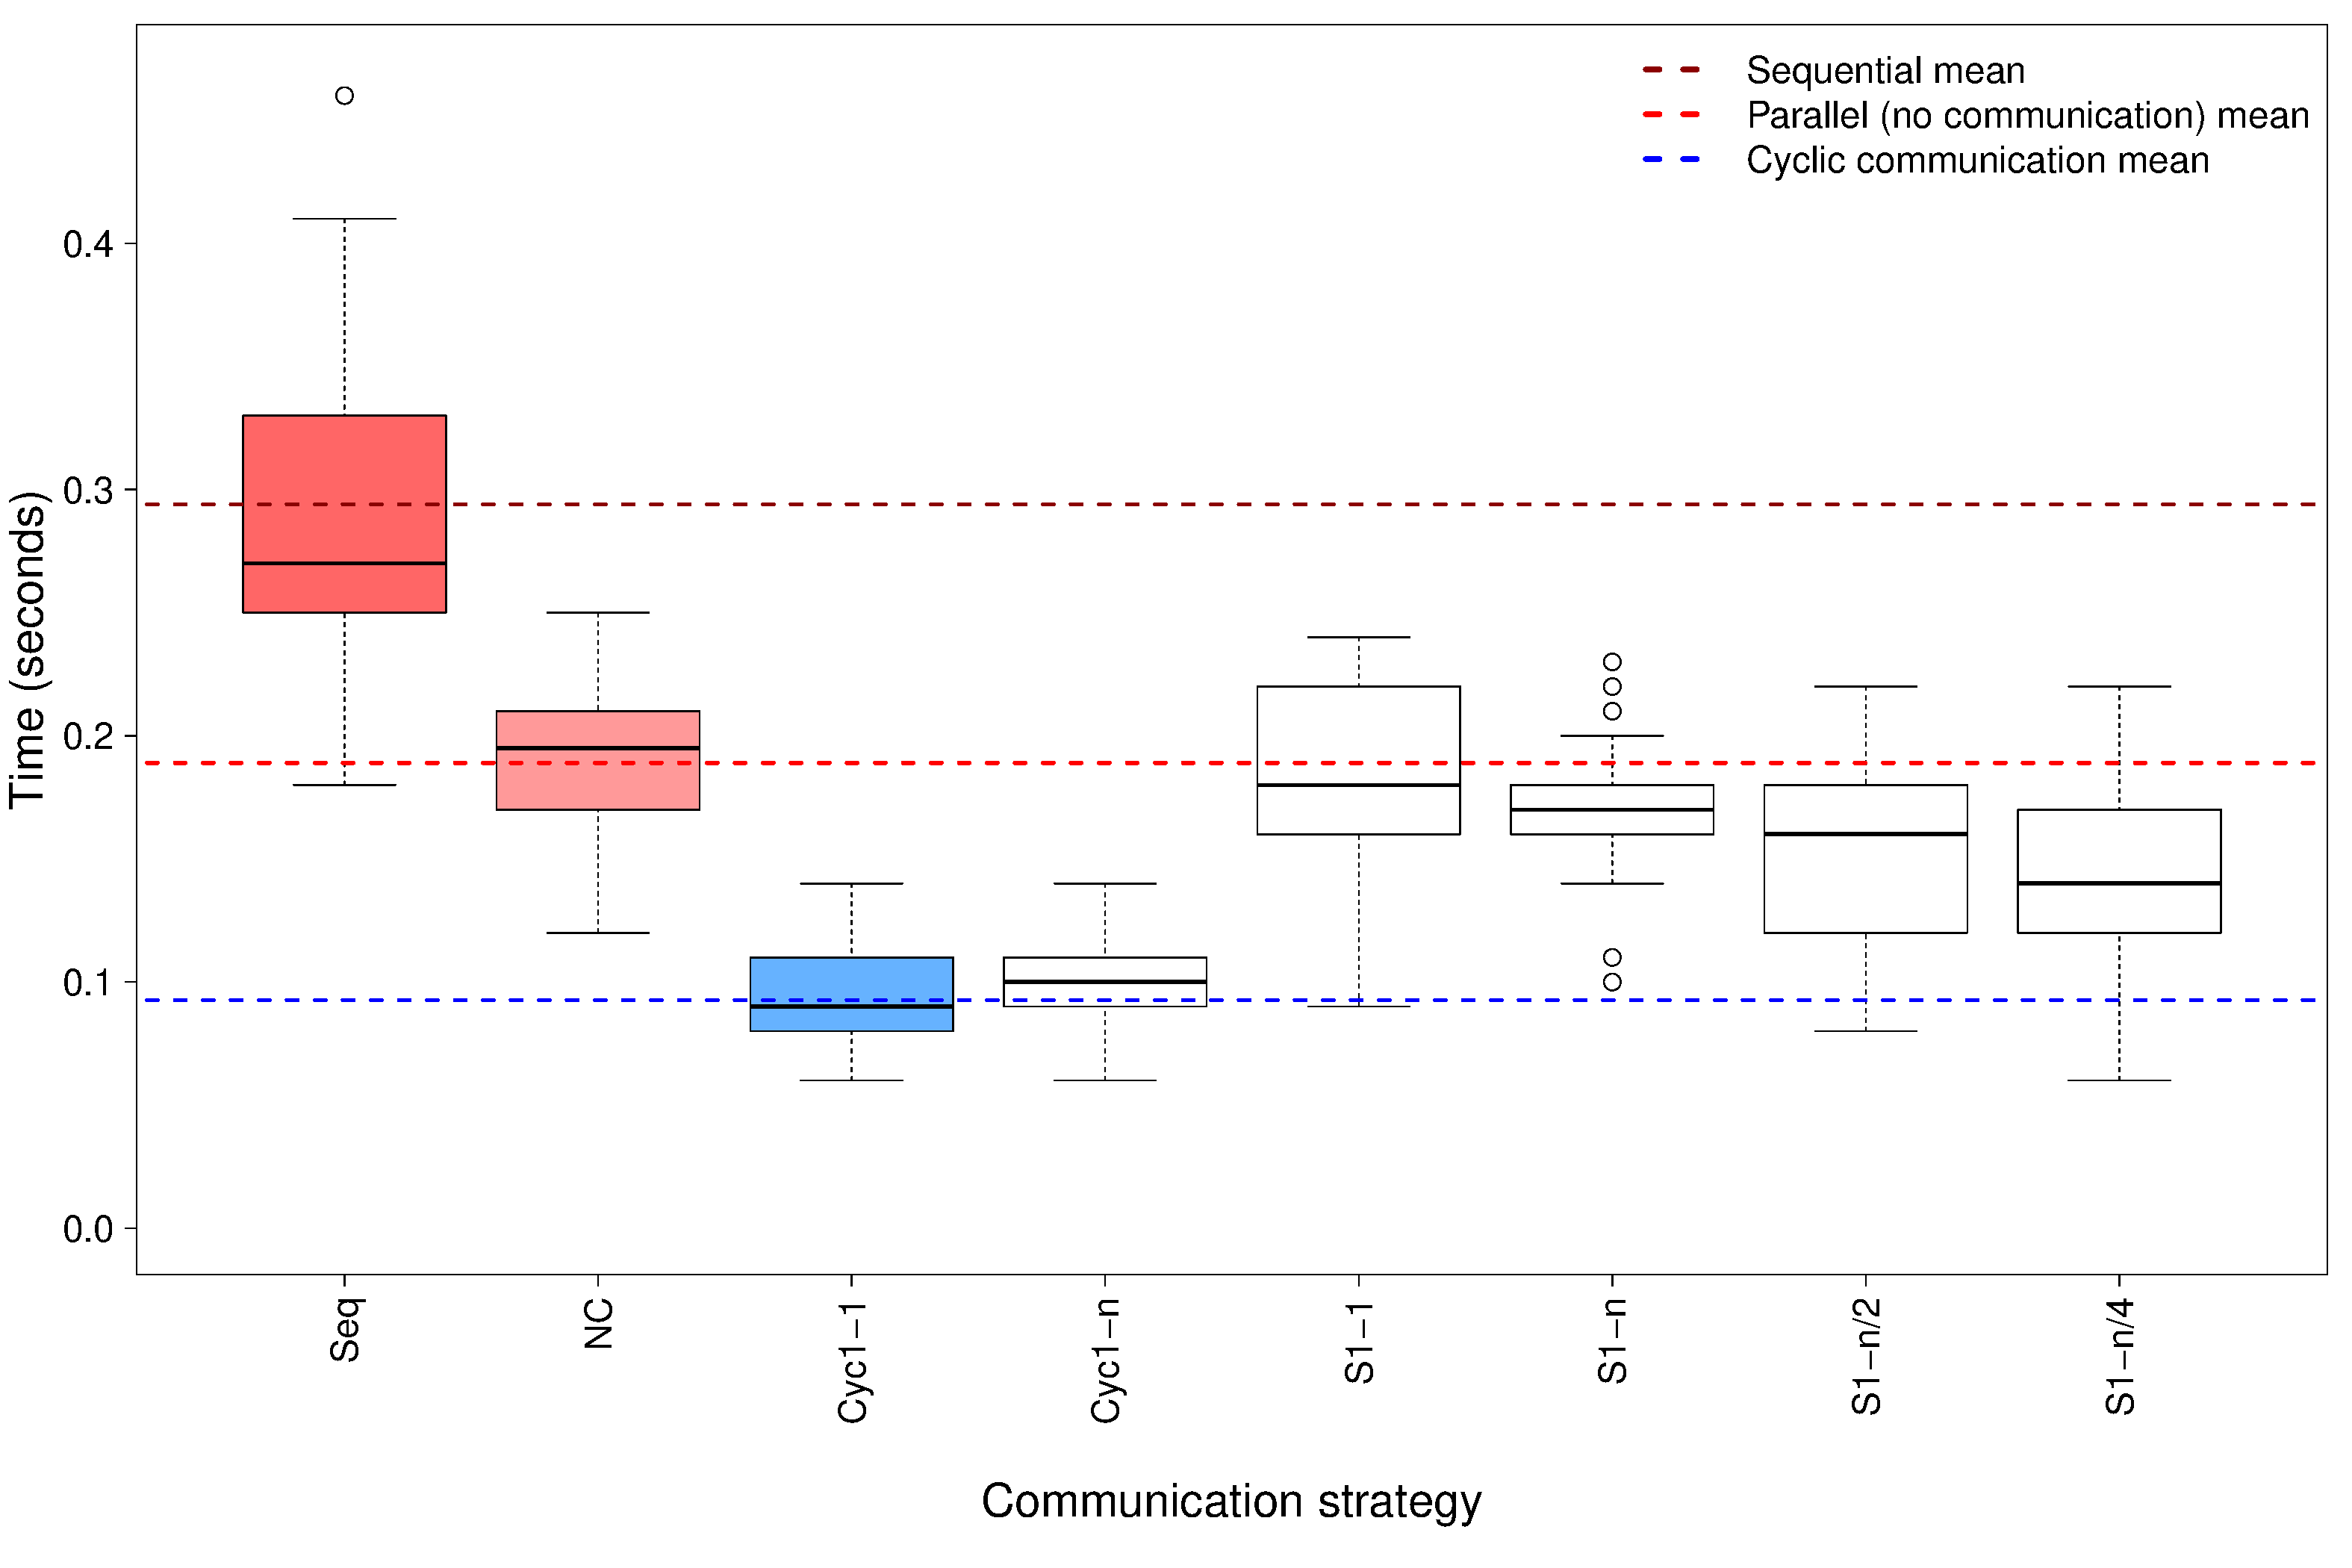
\includegraphics[width=0.35\textwidth]{nq250_BP.pdf}
%\caption{Different communication strategies to solve 250-Queens using \posl}\label{boxplot:250_2}
%\end{figure}

\begin{minipage}[c]{0.45\textwidth}
\centering
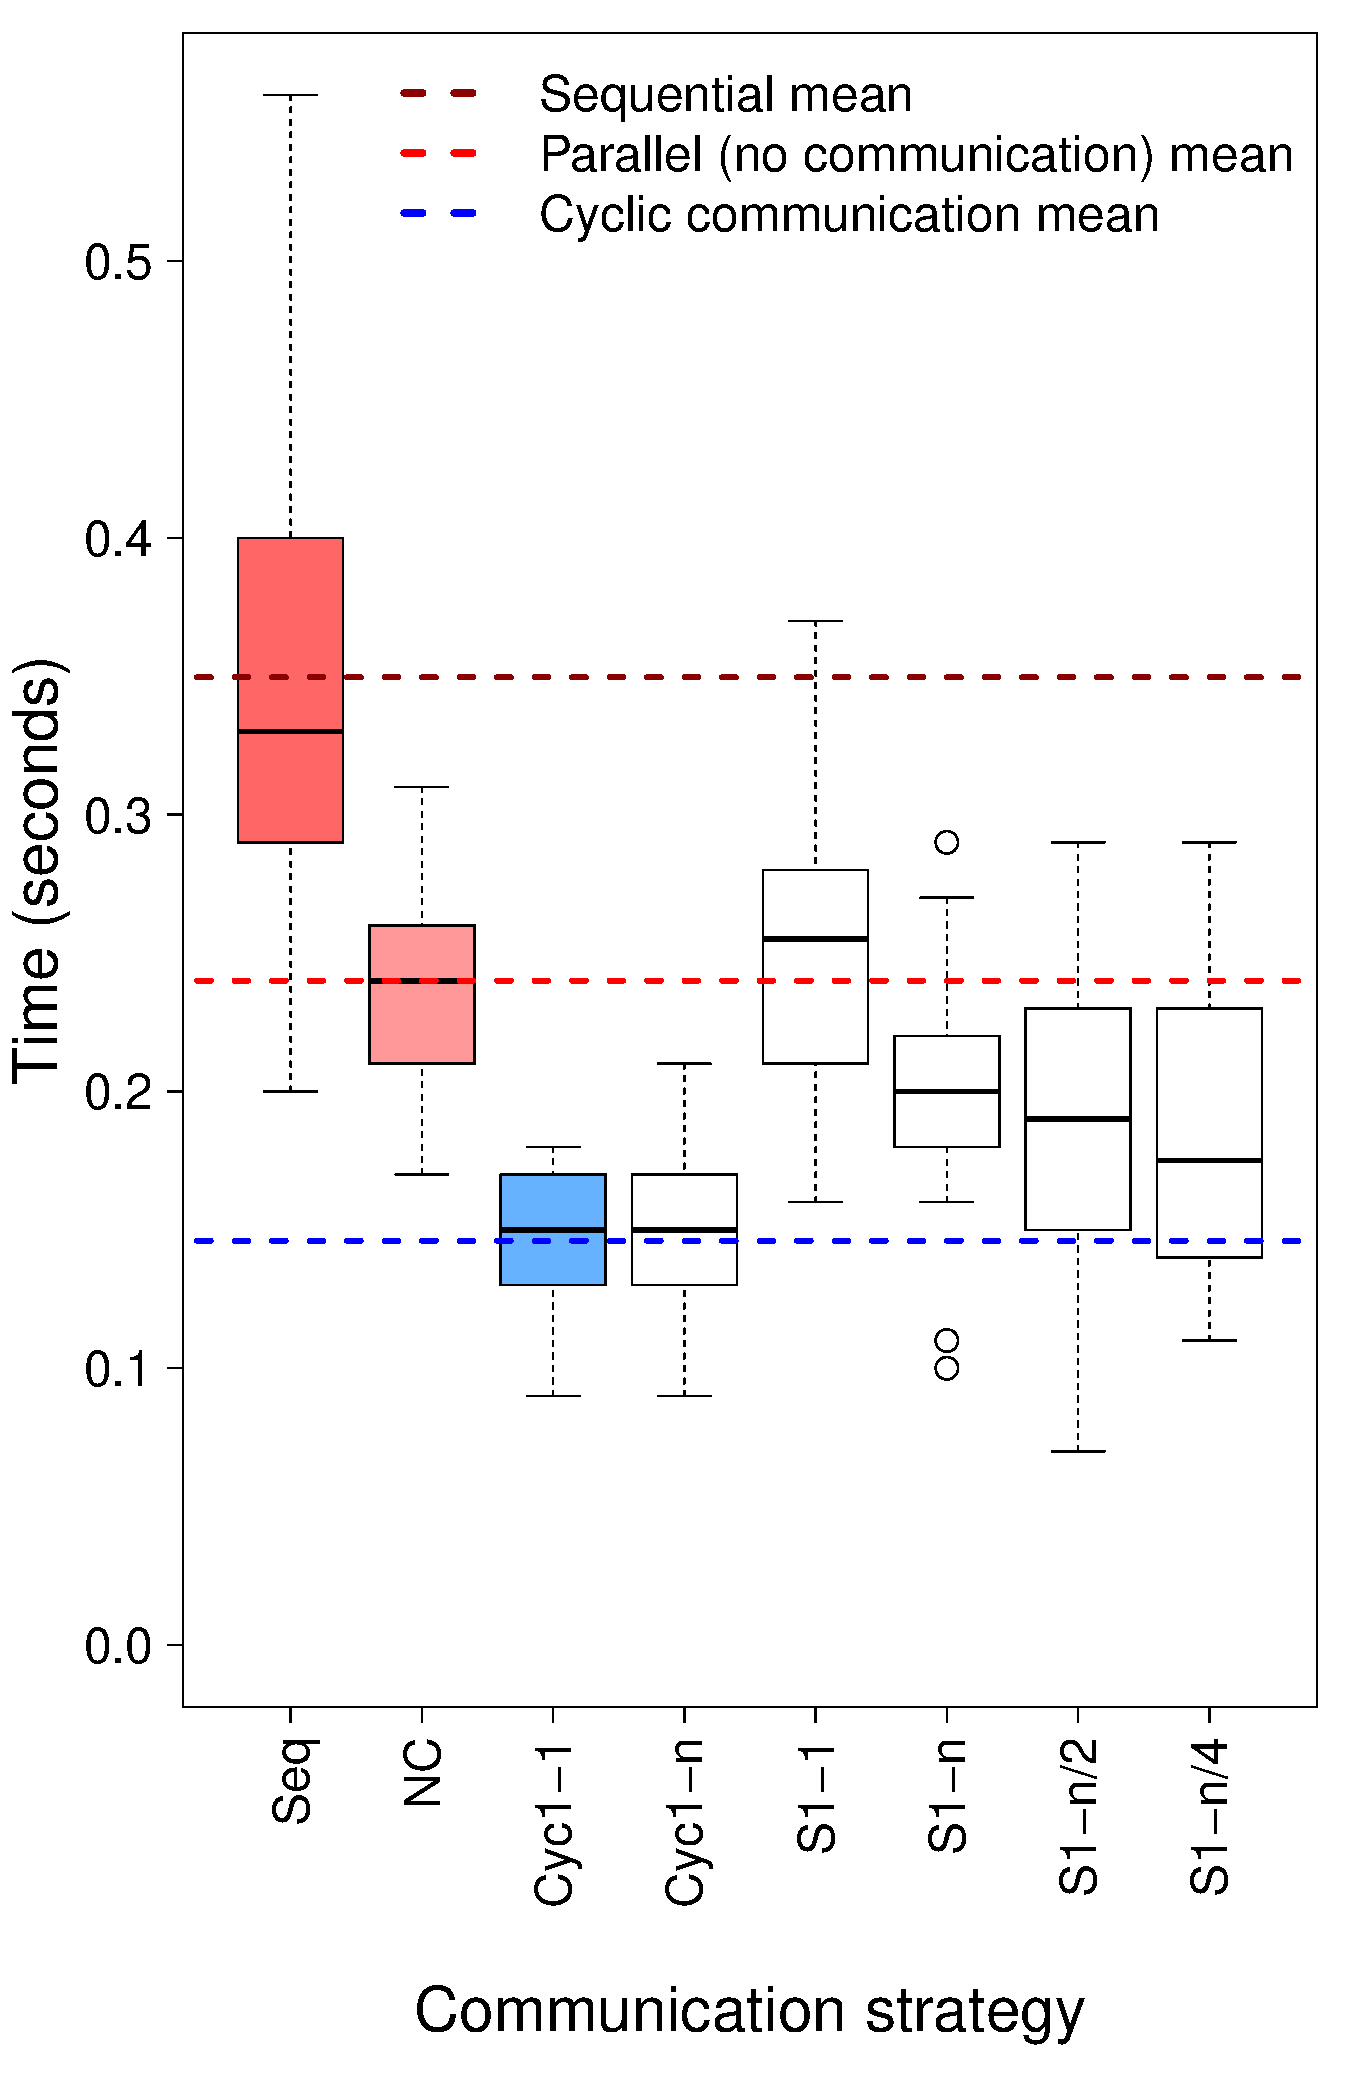
\includegraphics[width=0.8\textwidth]{nq500_BP.pdf}
\captionof{figure}{Different communication strategies to solve 500-Queens using \posl}\label{boxplot:500}
\end{minipage}\hspace{0.05\textwidth}
\begin{minipage}[c]{0.45\textwidth}
\centering
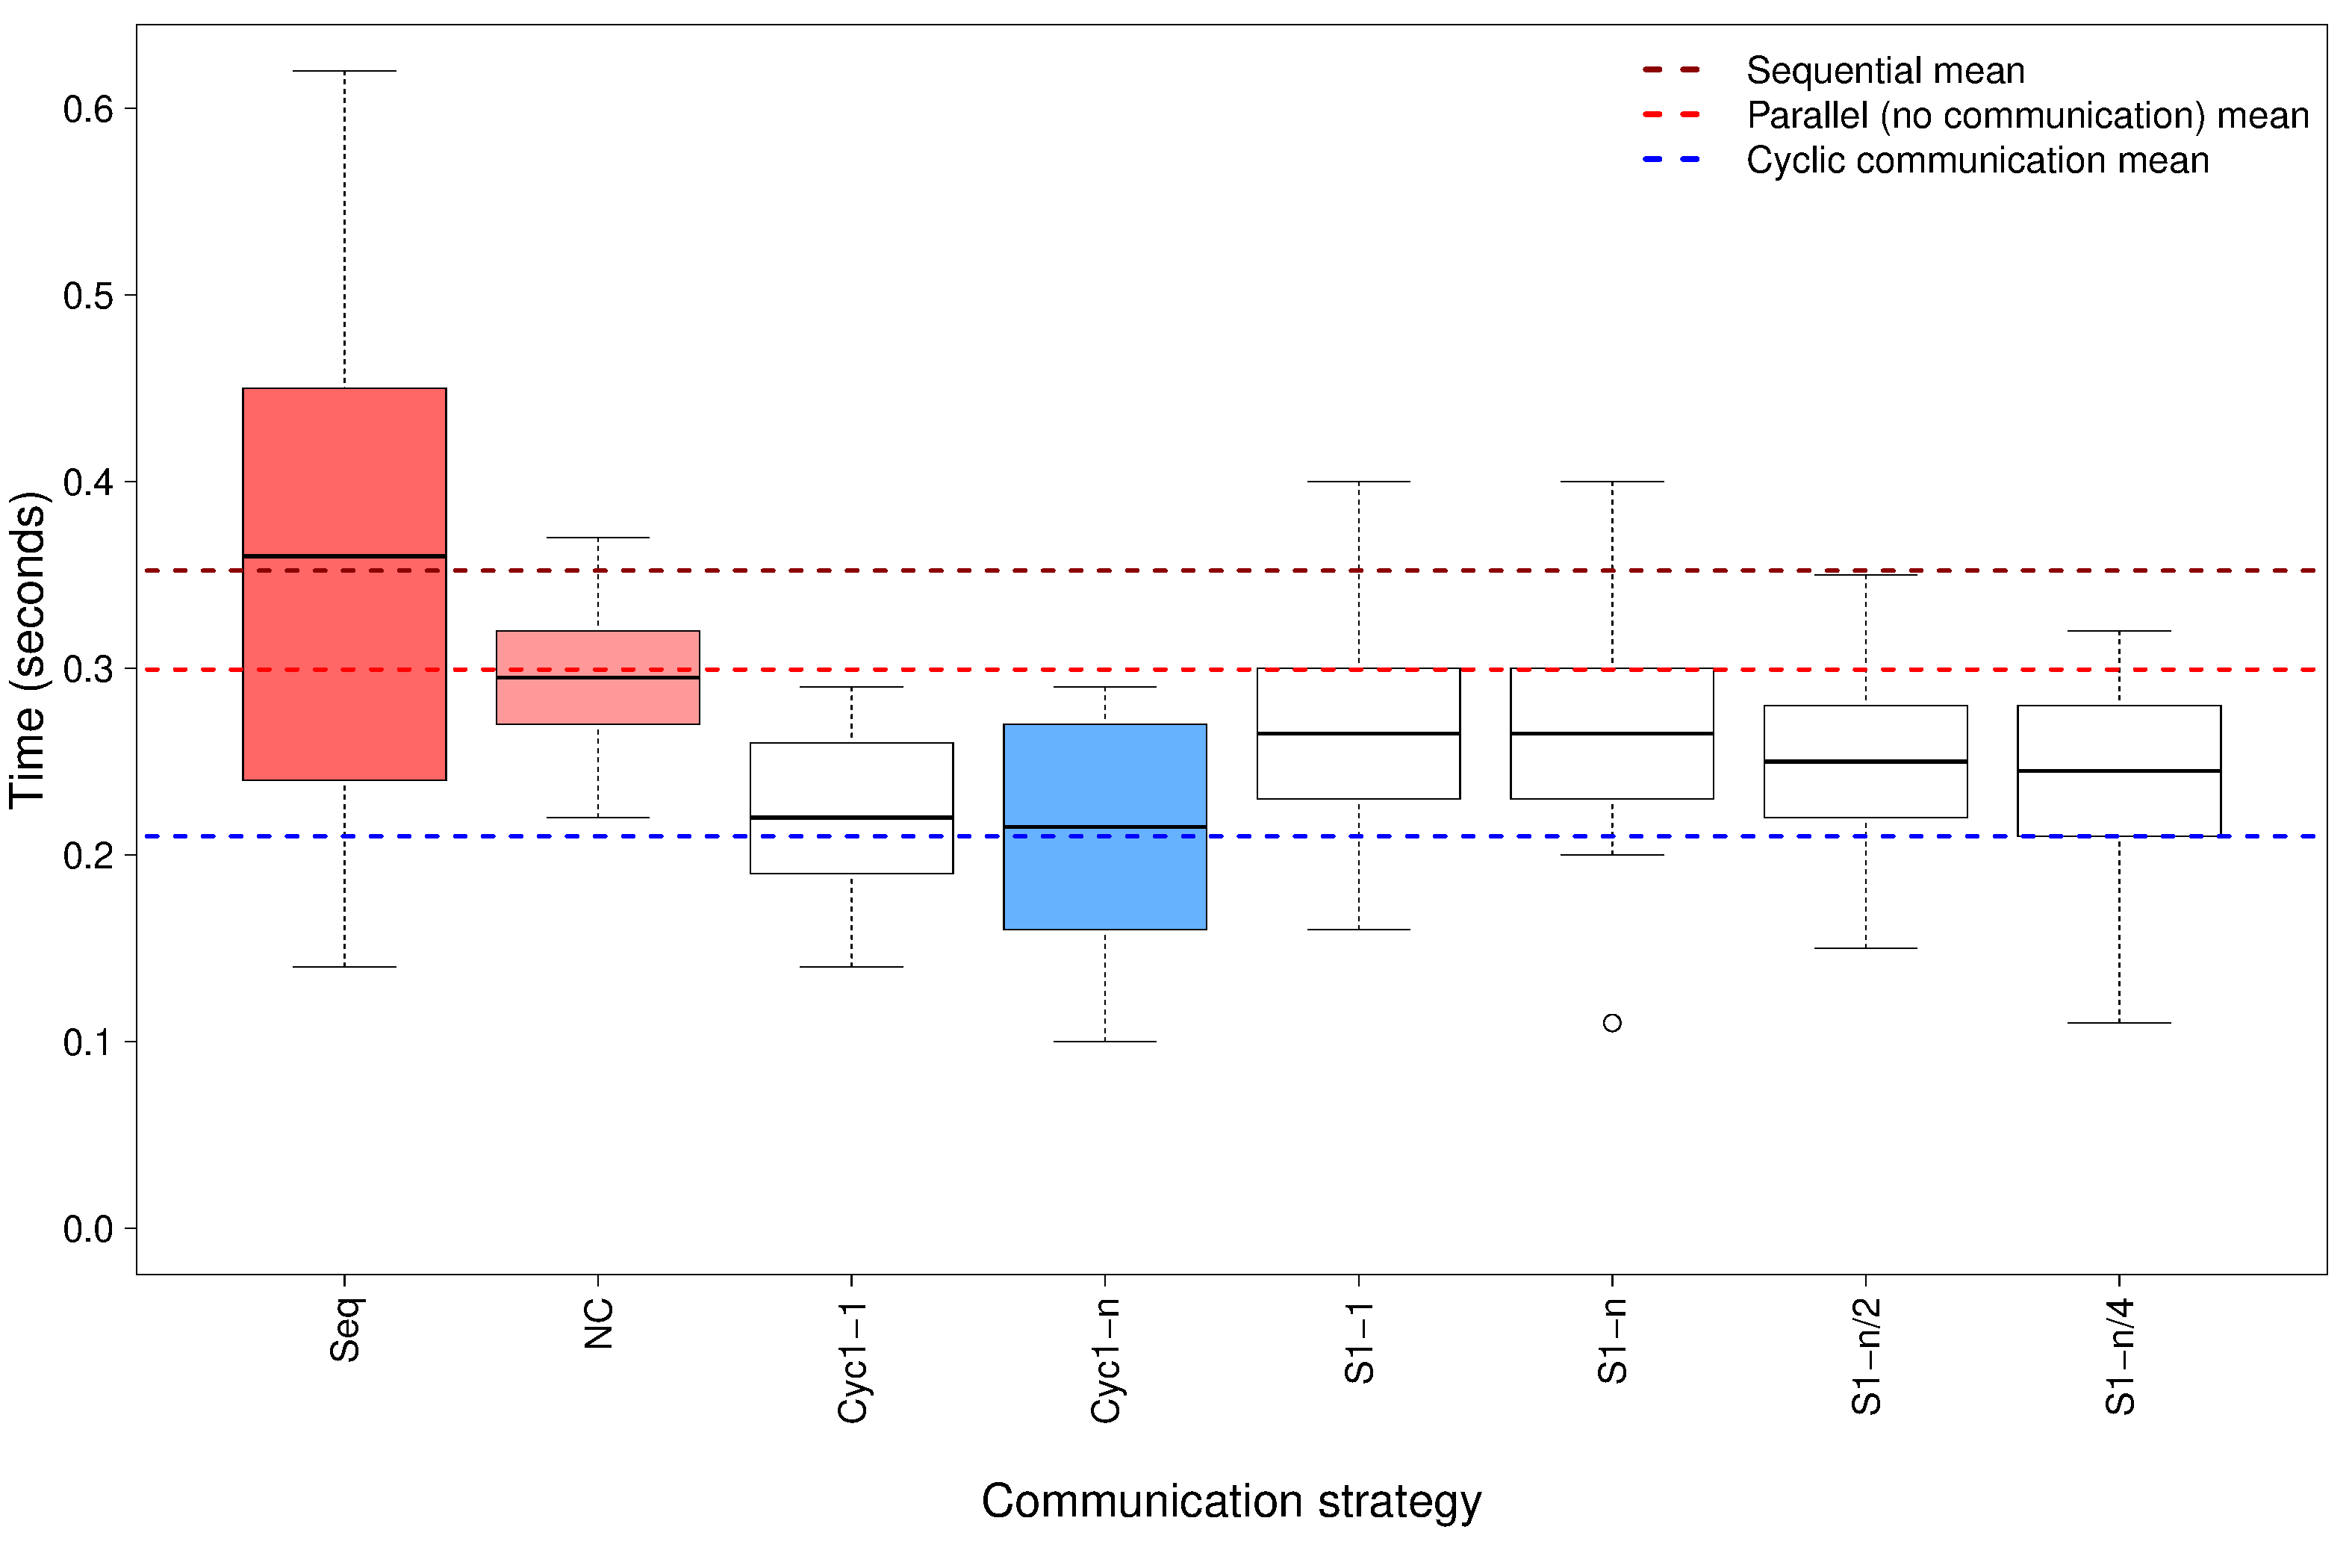
\includegraphics[width=0.8\textwidth]{nq1000_BP.pdf}
\captionof{figure}{Different communication strategies to solve 1000-Queens using \posl}\label{boxplot:1000}
\end{minipage}

\begin{figure}[!h]
\centering
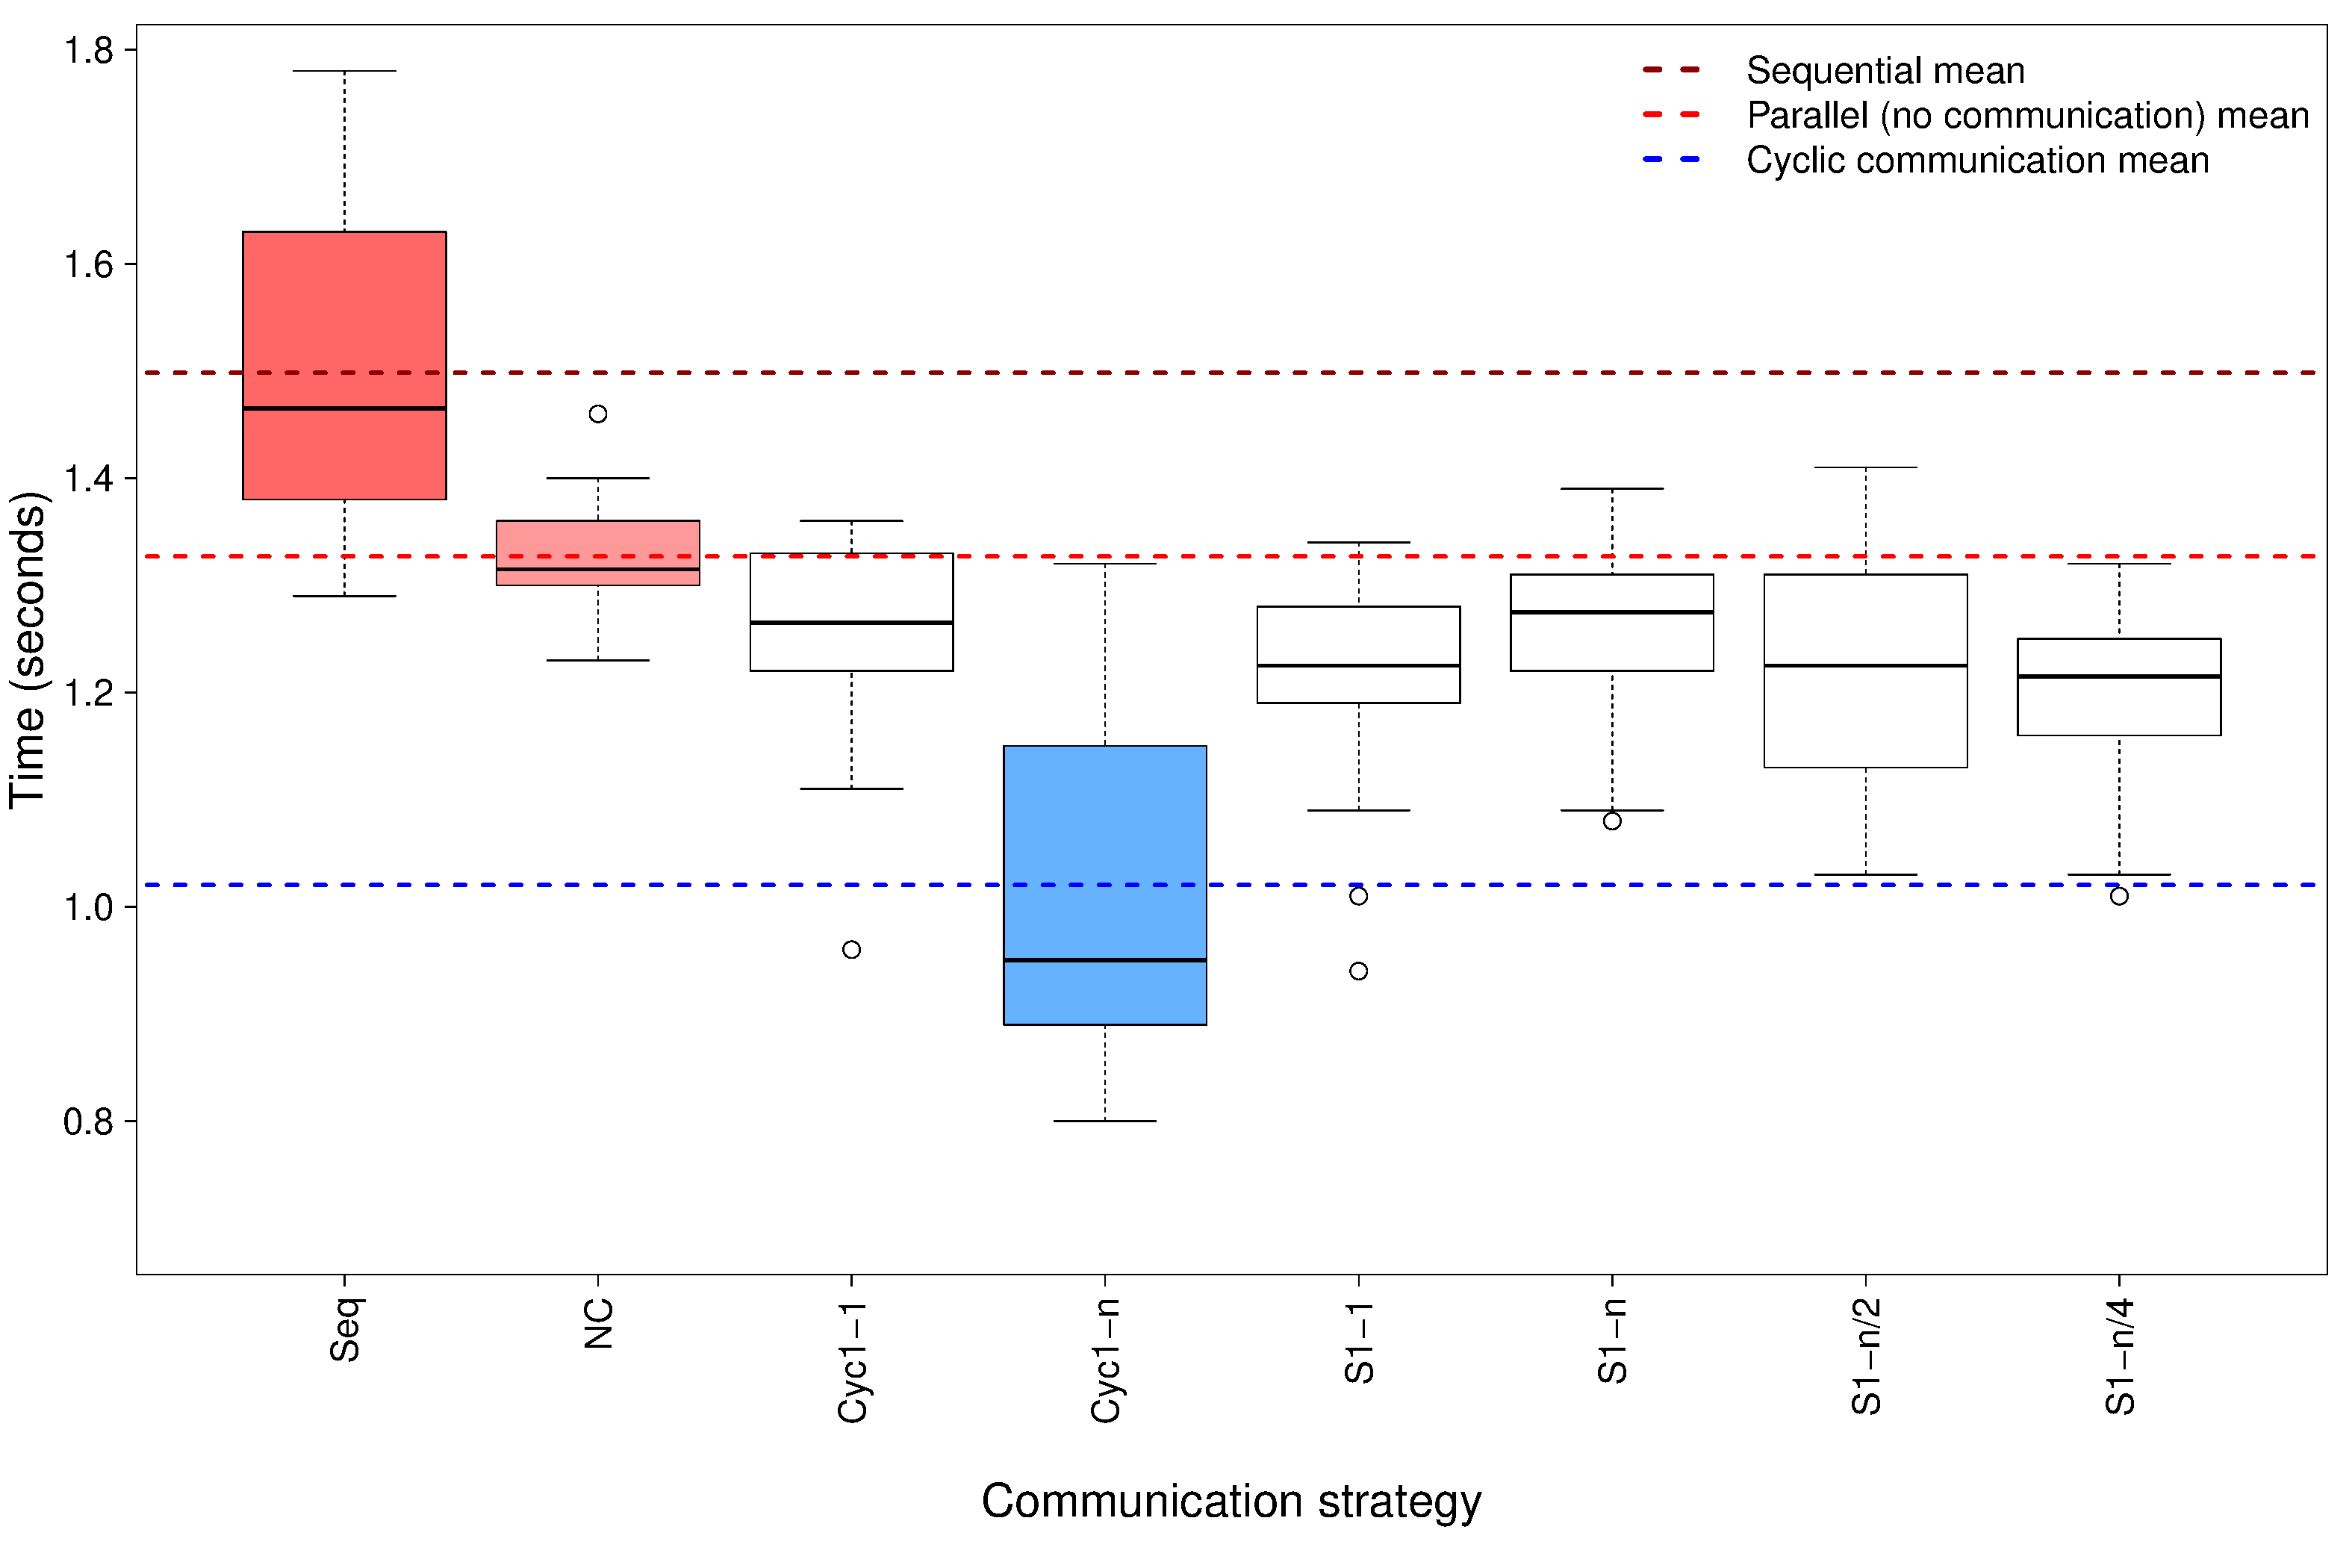
\includegraphics[width=0.35\textwidth]{nq3000_BP.pdf}
\caption{Different communication strategies to solve 3000-Queens using \posl}\label{boxplot:3000}
\end{figure}

\begin{figure}[!h]
\centering
\includegraphics[width=0.8\textwidth]{nq6000_BP_big.pdf}
\caption{Different communication strategies to solve 6000-Queens using \posl}\label{boxplot:6000}
\end{figure}

\newpage

\section{Winner solver type representation}

Figures~\ref{barplot:250}, \ref{barplot:500}, \ref{barplot:1000}, \ref{barplot:3000} and \ref{barplot:6000}, represent the percentage of winner solvers for each communication strategy, according to three different types:

\poslcaptiondesciption{
\begin{tabular}[t]{rl}
\receiver{Receiver}: & Receiver solver wining thanks to the received information \\
\sender{Sender}: & Sender solver \\
\nonreceiver{Passive receiver}: & Receiver solver wining without using the received information \\
%\textbf{Non communicating}: & Non communicating solver \\
\end{tabular}
}

Bar graphs in this section provide a clear evidence that the communication has played an important role during the solution process. They are also a different point of view to observe how the number of winner receiver solvers decrease along with the order of the problem, i.e. the communication is less effective.

%-------- SOLVER TYPE
\begin{figure}[!h]
\centering
\subfloat[][\NQP{} 250 ]{
	\label{barplot:250}
	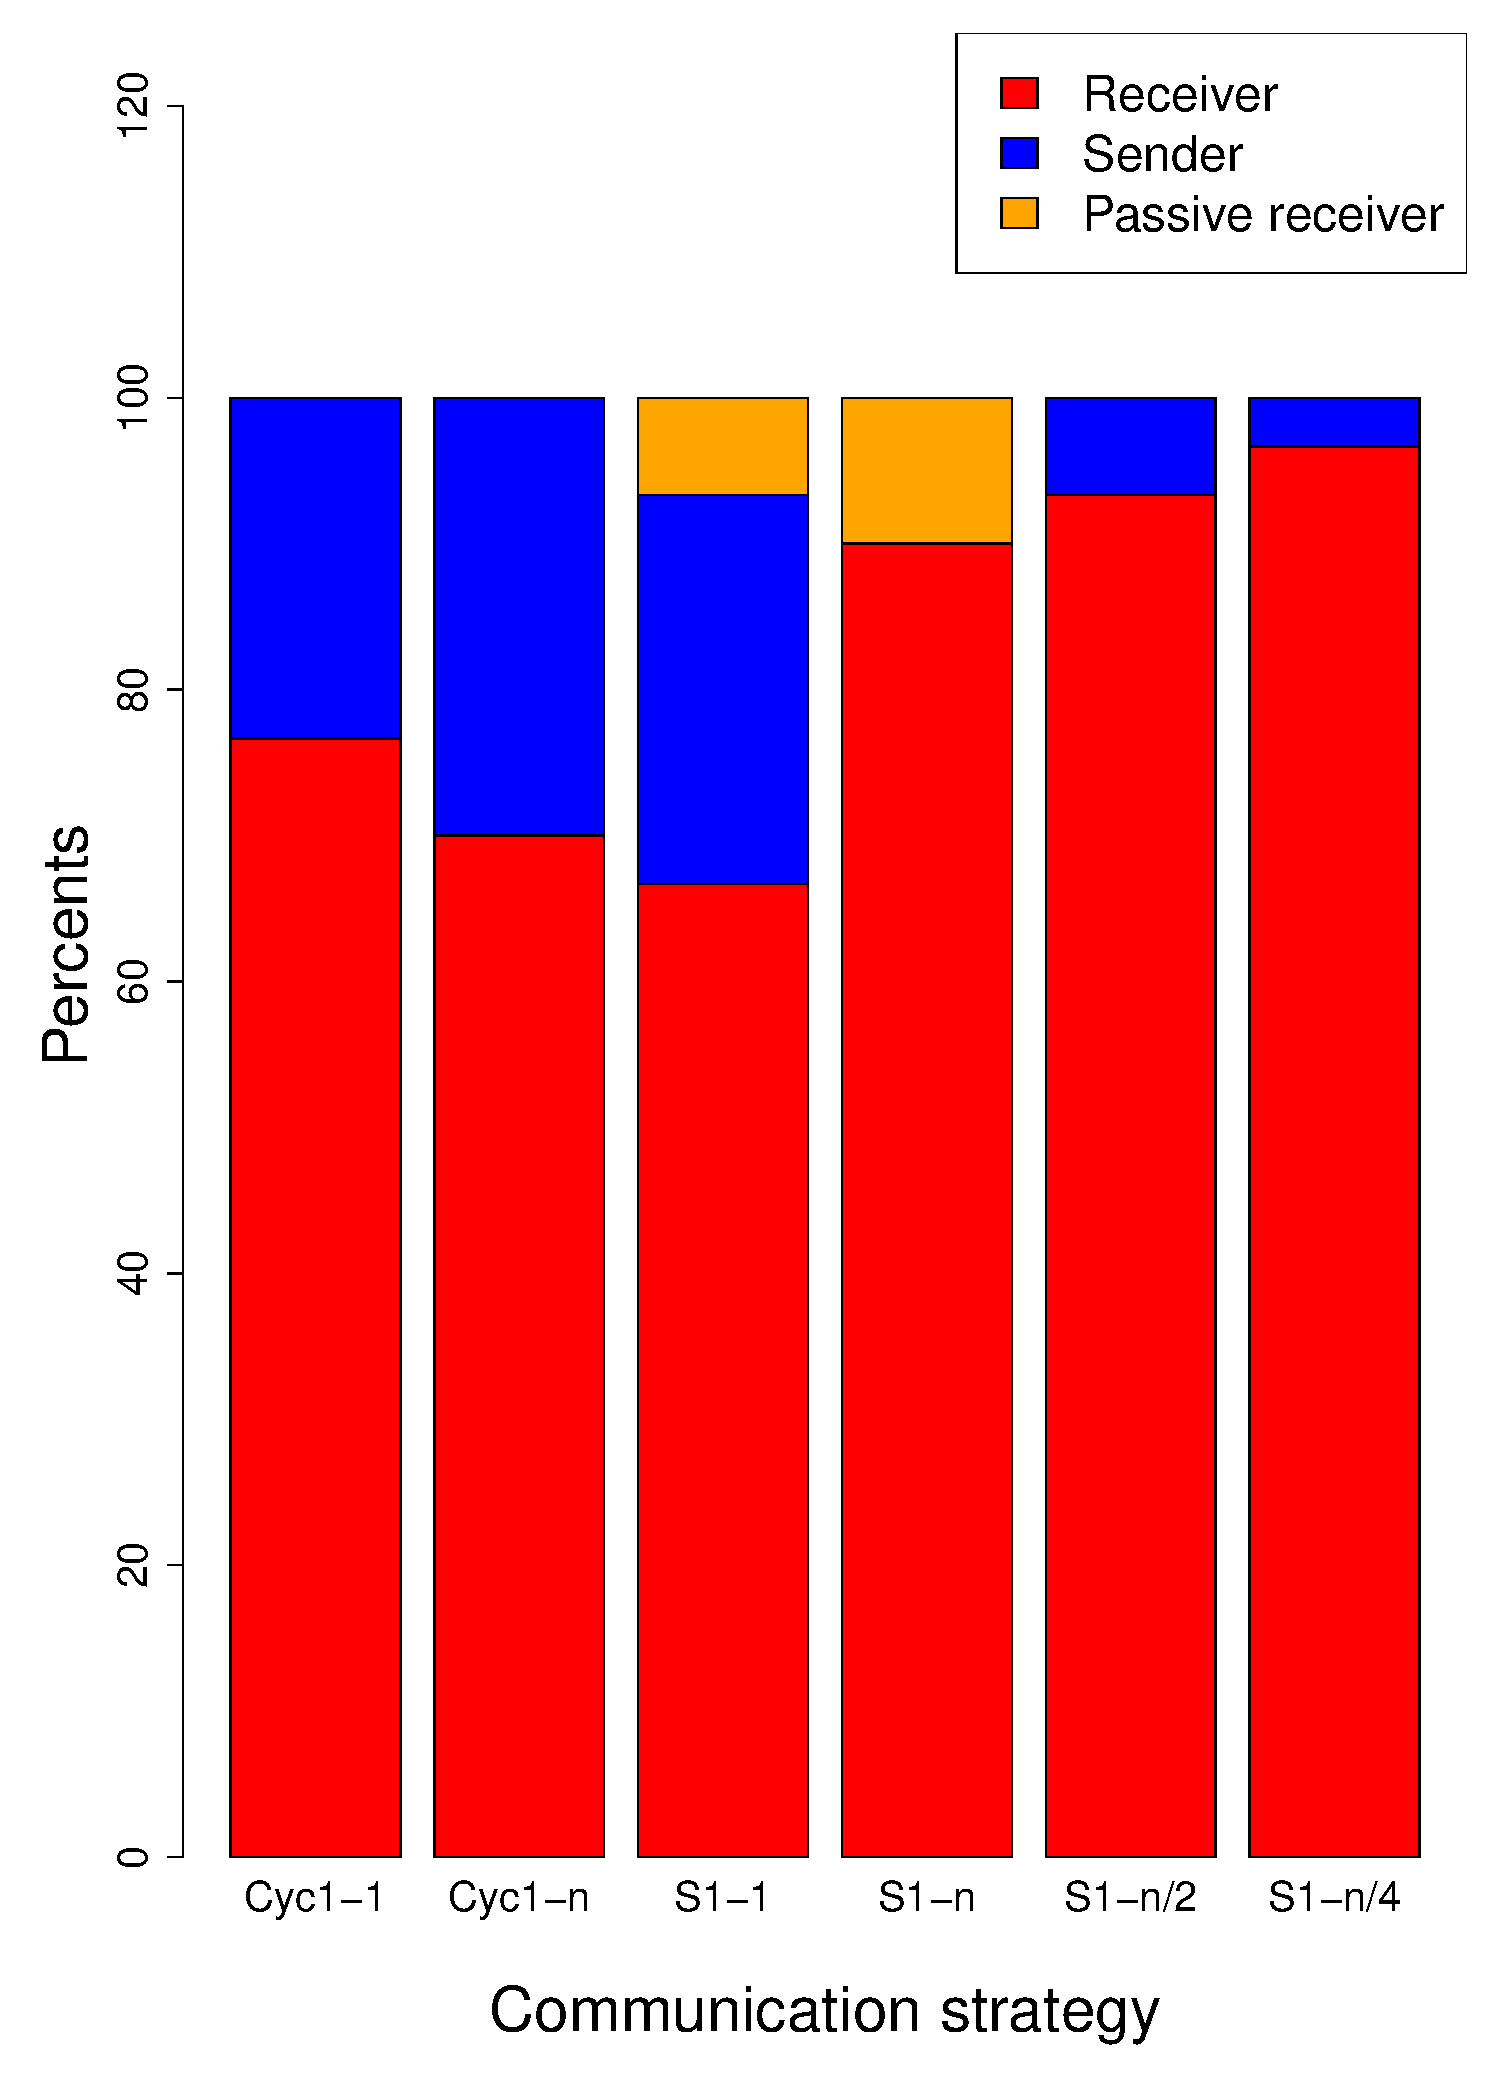
\includegraphics[width=0.5\linewidth]{nq250_per_BP.pdf}
} %\hspace{0.05\linewidth}
\subfloat[][\NQP{} 500 ]{%
	\label{barplot:500}
	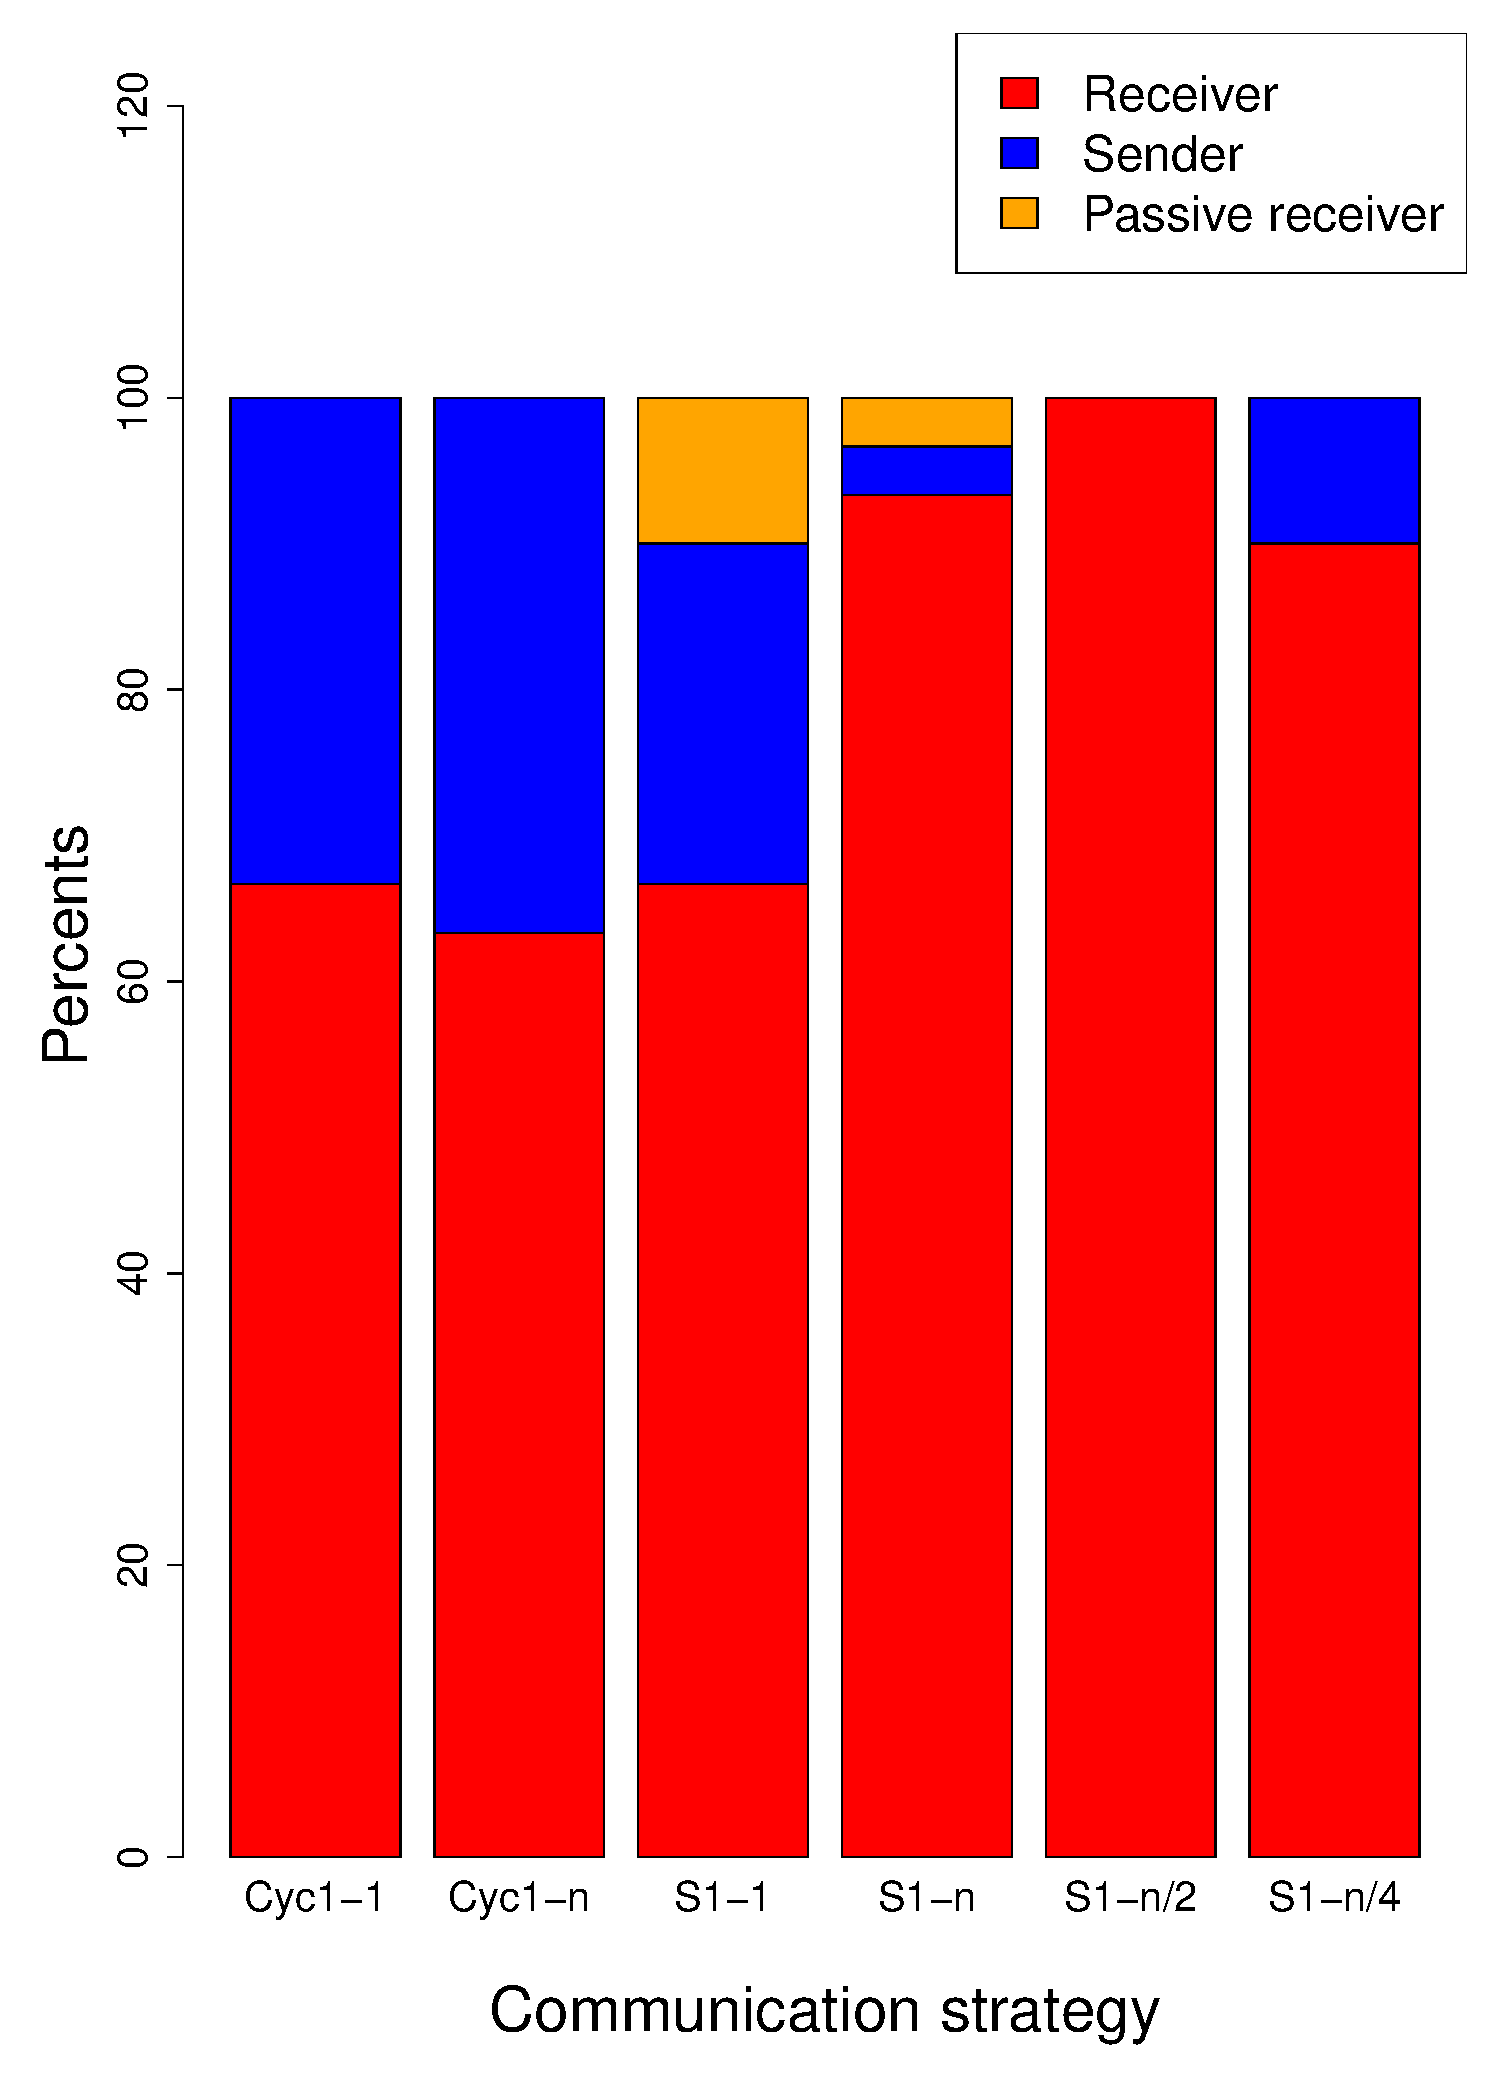
\includegraphics[width=0.5\linewidth]{nq500_per_BP.pdf}
}\\
\subfloat[][\NQP{} 1000 ]{
	\label{barplot:1000}
	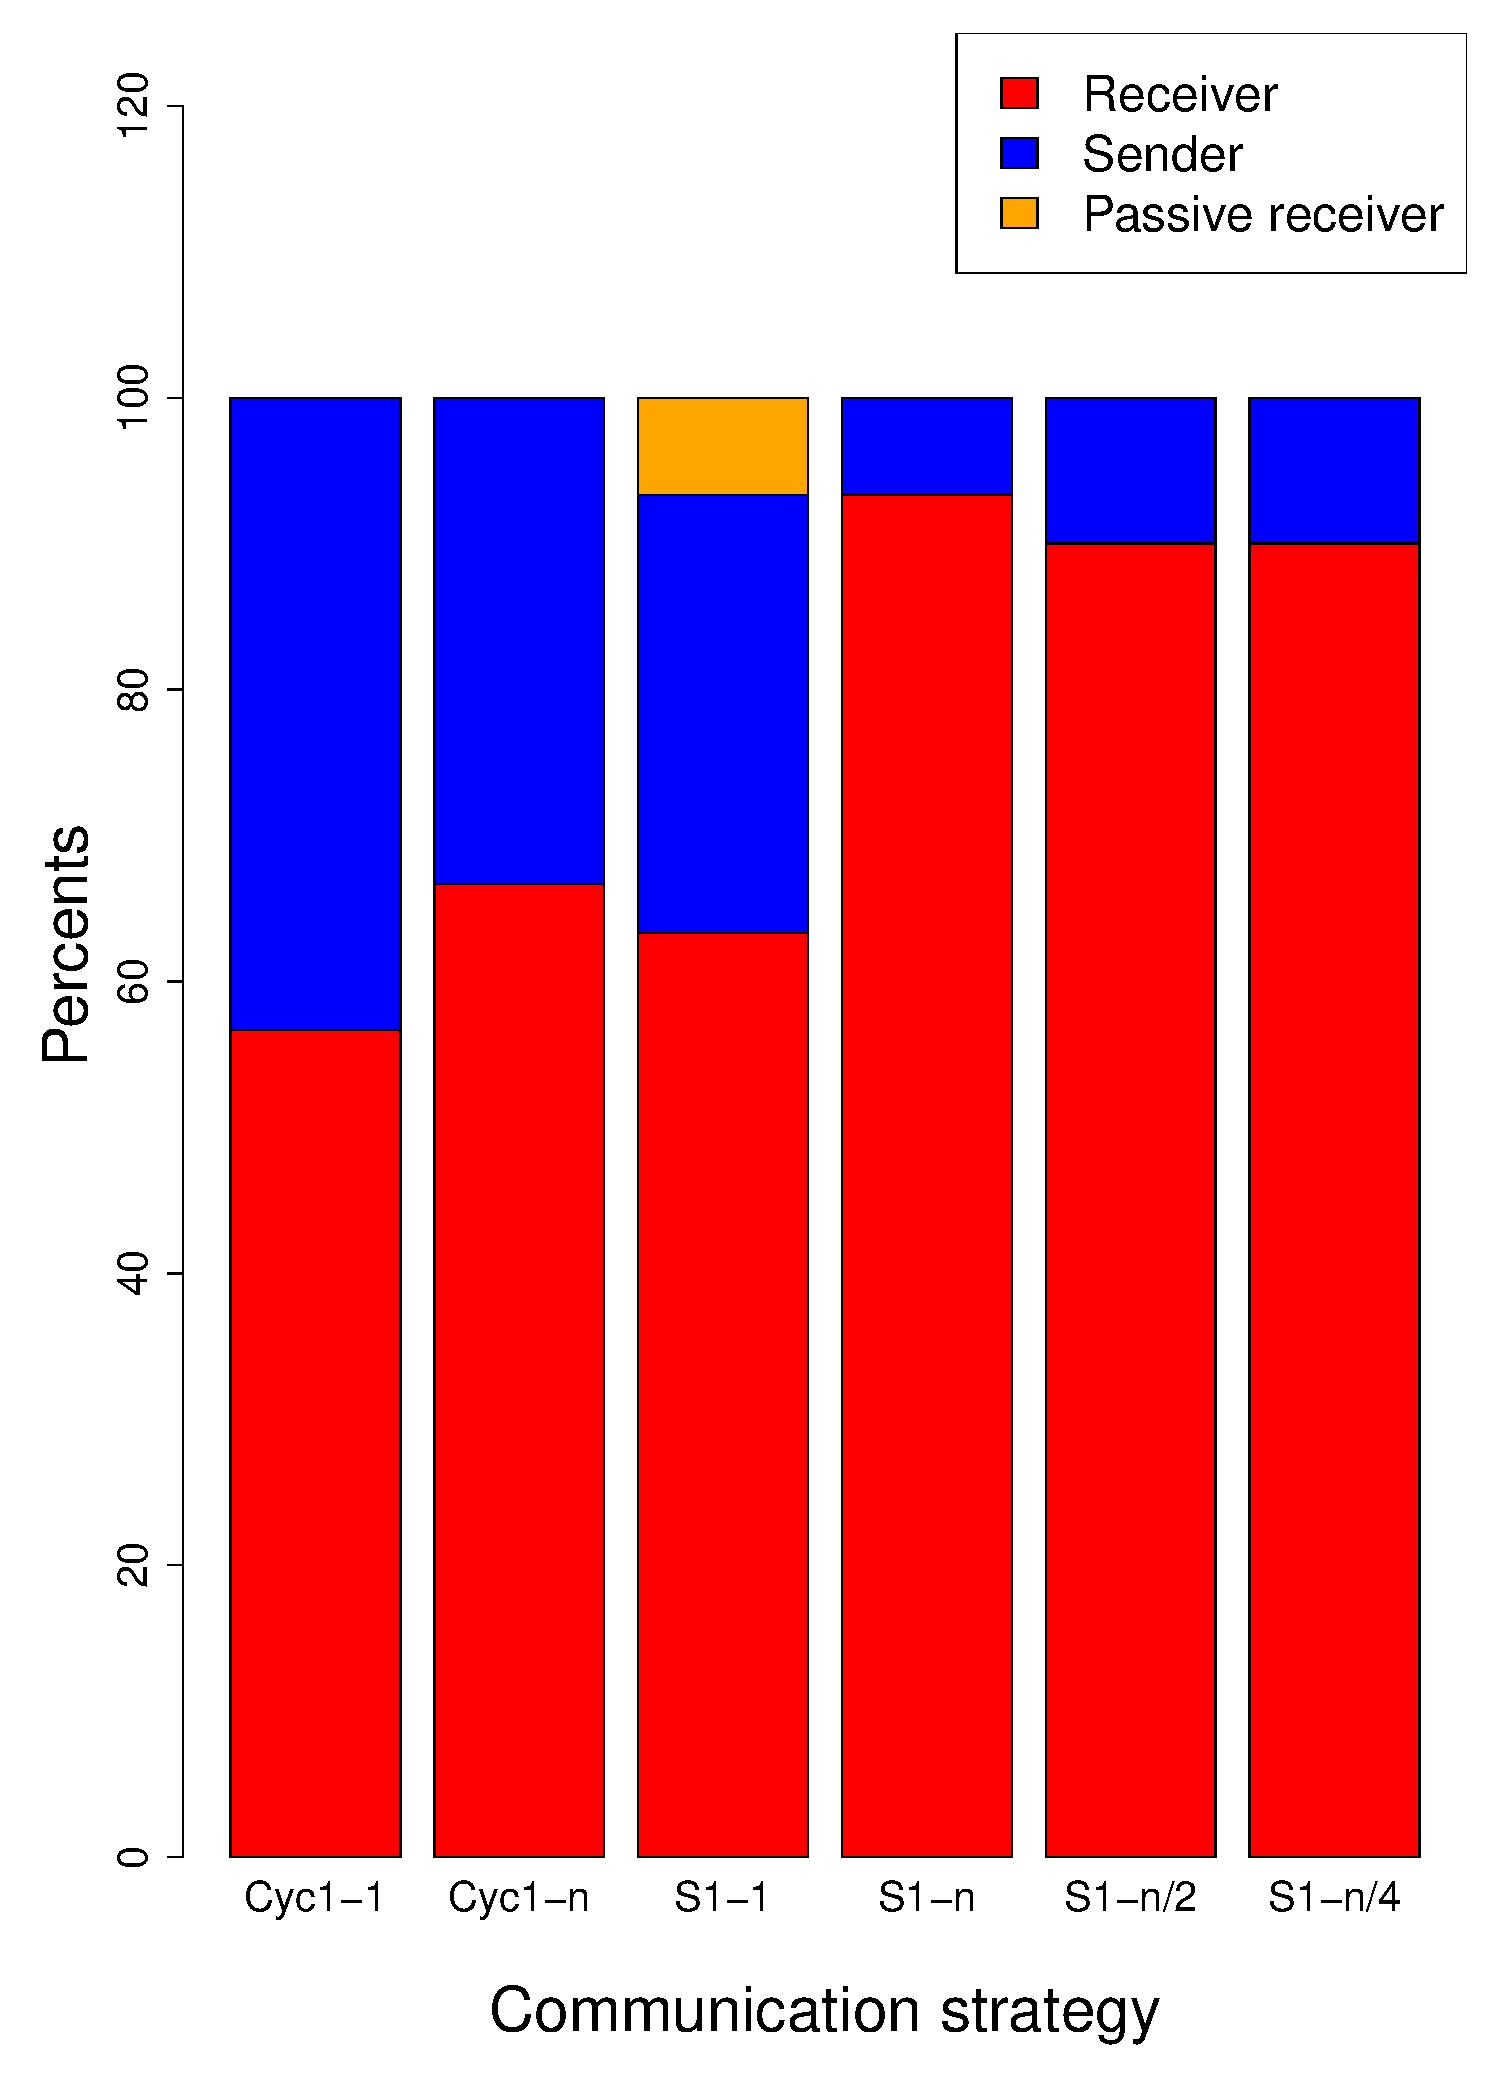
\includegraphics[width=0.5\linewidth]{nq1000_per_BP.pdf}
} %\hspace{0.05\linewidth}
\subfloat[][\NQP{} 3000 ]{%
	\label{barplot:3000}
	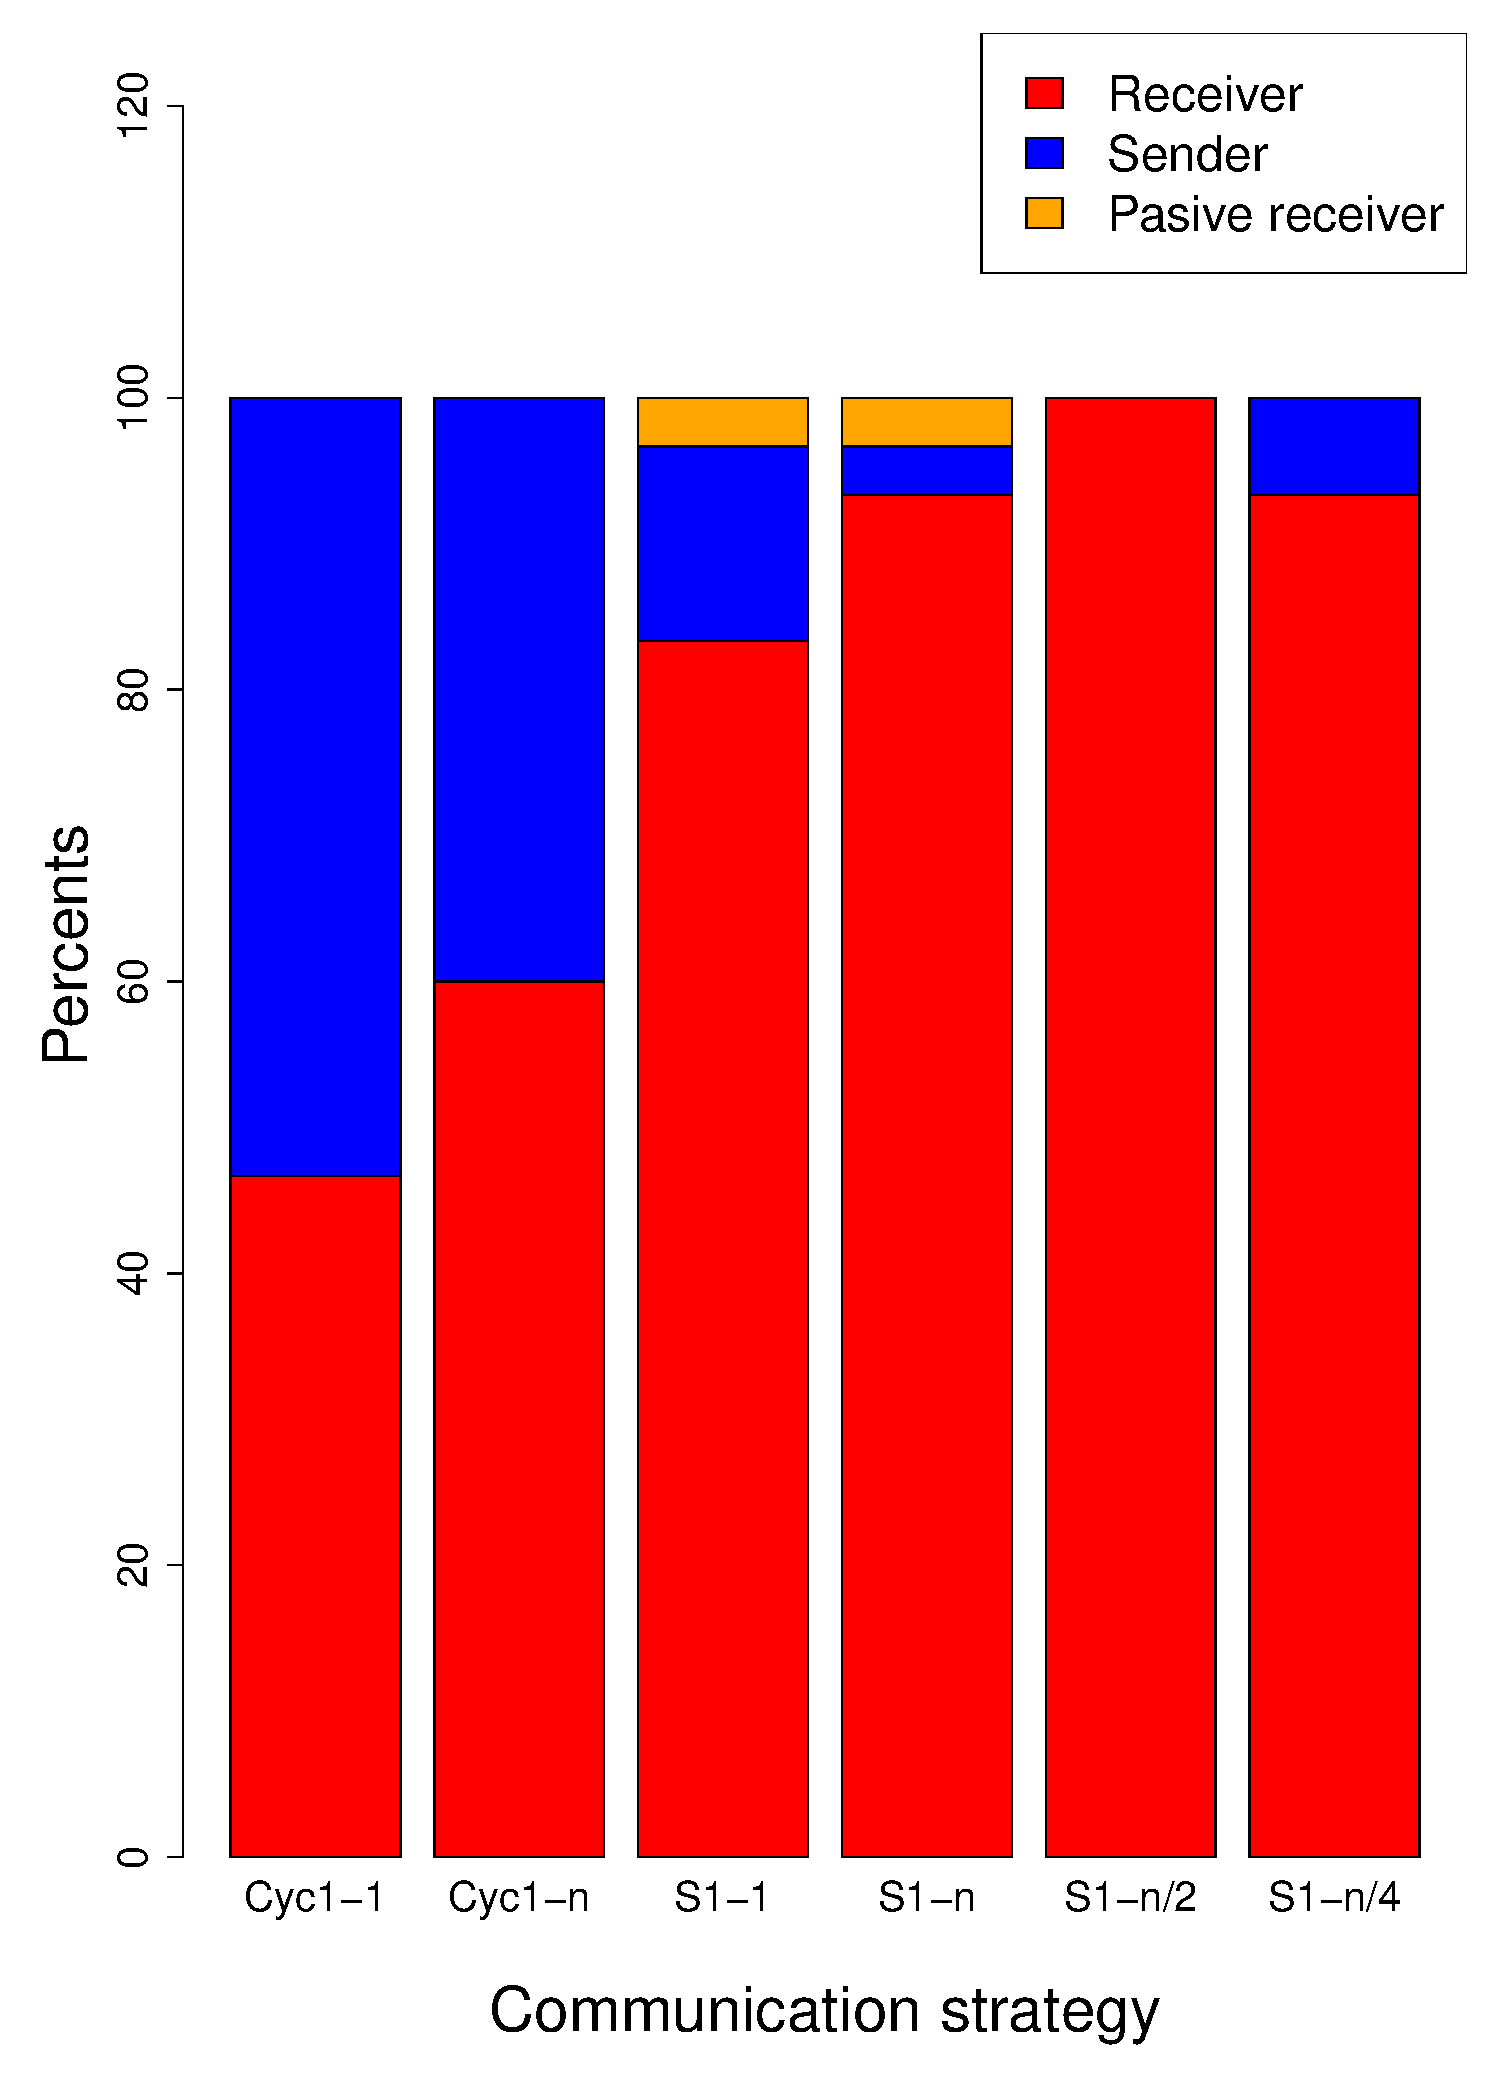
\includegraphics[width=0.5\linewidth]{nq3000_per_BP.pdf}
}
\caption[]{Solver proportion for each communication strategy to solve \NQP{} using \posl}
\label{fig:bars_nq}
\end{figure}

\begin{figure}[!h]
\centering
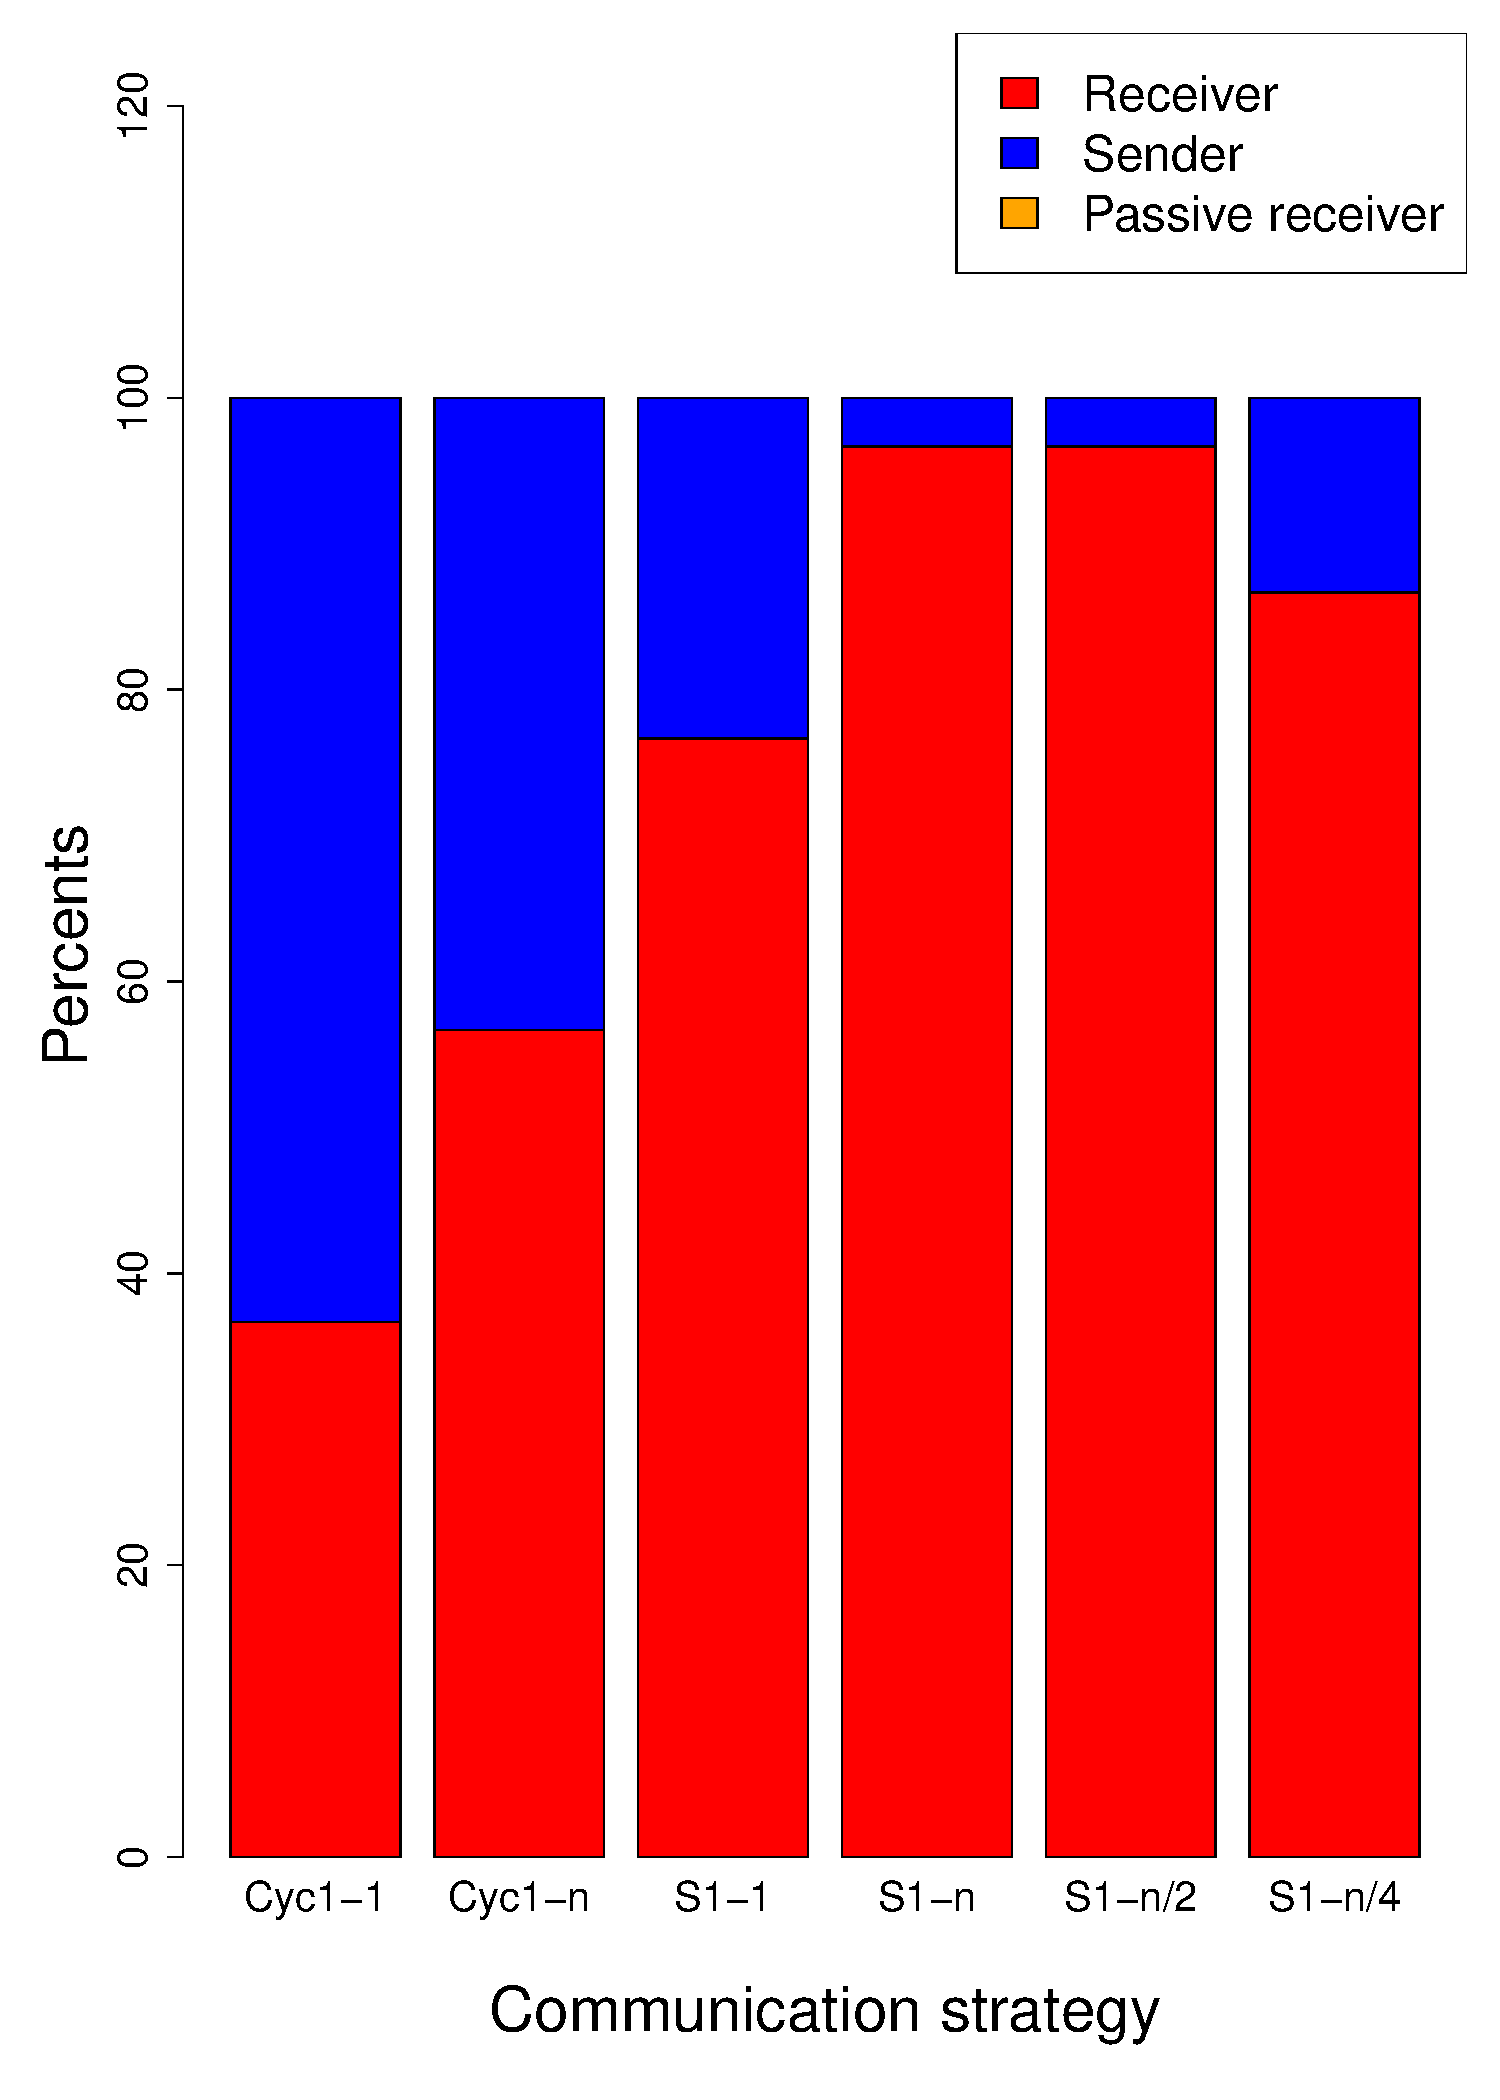
\includegraphics[width=0.5\textwidth]{nq6000_per_BP.pdf}
\caption{Solver proportion for each communication strategy to solve \NQP{} using \posl}\label{barplot:6000}
\end{figure}